\Chapter{Mintaalkalmazás specifikáció}

Egy MMA harcosokkal foglalkozó weboldal, ami megvalósítja a RESTful API-t, képes CRUD műveleteket végrehajtani a harcosokon, mint létrehozás, beolvasás, frissítés és törlés. A harcosok listáját egy kereső mezővel lehet szűrni, így változik az oldalon megjelenített lista a beírt szó hatására. Ha a harcos neve tartalmazza a beírt betűsorozatot, akkor benne marad a listában, ha nem akkor kikerül belőle.

Új harcost az ,,Add new fighter'' feliratú gombbal lehet hozzáadni. Egy harcosnak a következő adatait lehet megadni:

\begin{itemize}
\item \textit{név}: A harcos teljes neve, minimum 3 karakter hosszúságúnak kell lennie. Megadása kötelező. Szöveg mező.
\item \textit{becenév}: A harcos beceneve, nem kötelező megadni. Szöveg mező.
\item \textit{súlycsoport}: Az előre megadott súlycsoportok közül a harcos súlycsoportjának kiválasztása, megadása kötelező, választási lehetőség: 5. Szöveg mező.
\item \textit{születési dátum}: A harcos születési dátuma: év, hónap, nap formátumban, megadása kötelező. Dátum mező.
\item \textit{szülőváros}: A harcos szülőváros, nem kötelező megadni. Szöveg mező.
\item \textit{nemzetiség}: A harcos nemzetisége: minimum 2 karakter, megadása kötelező. Szöveg mező.
\item \textit{magasság}: A harcos magassága centiméterben értve, 155 és 205 közé kell, hogy essen, megadása kötelező. Szám mező.
\item \textit{súly}: A harcos súlya kilogrammban értve, 50 és 120 közé kell, hogy essen, megadása kötelező.  Szám mező.
\item \textit{record}: A harcos rekordja Győzelem-Döntetlen-Vereség formában, megadása kötelező. 
\item \textit{harcos avatárjának URL linkje}: Szöveg mező, megadása kötelező.
\item \textit{a harcossal foglalkozó oldal URL linkje}: Szöveg mező, nem kötelező megadni.
\end{itemize}

A harcosok a főoldalon (home) lévő „VIEW THE FIGHTERS” elnevezésű gombra kattintva jelennek meg. Minden harcos sorában egy „View Details” nevezetű kék gomb van, ami átirányít a ???????? oldalra, ahol megtekinthetők az adott harcos további adatai. Továbbá ezen az oldalon tudjuk frissíteni az adatokat az Edit gombra kattintva.

Törölni a „Delete” nevű gombbal lehet. A Go Back nevezetű gombbal a harcosokat megjelenítő oldalra tudunk visszanavigálni. A kitöltendő űrlap (form) az „Create” (létrehozás) esetén validációval van ellátva. A fent említett táblázatban szerepelnek a kitöltendő mezők leírásai, illetve megadásuknak a megszorításai. A back-end szolgáltatást a MongoDB adatbázis, a Node.js, mint szerver és a legnépszerűbb Node.js keretrendszer, az Express biztosítja, ami a HTTP kérések irányításáért felel.

Front-end részről, mint személyes preferált keretrendszer az AngularJS és Angular 2. Ezek mellett még a ReactJS, a Backbone.js és a Vue.js.

Az alkalmazás elindítása és a sikeres bejelentkezés után ez a képernyő fogadja a felhasználót (\ref{fig:new_fighter}. ábra).

\begin{figure}[htb]
\centering
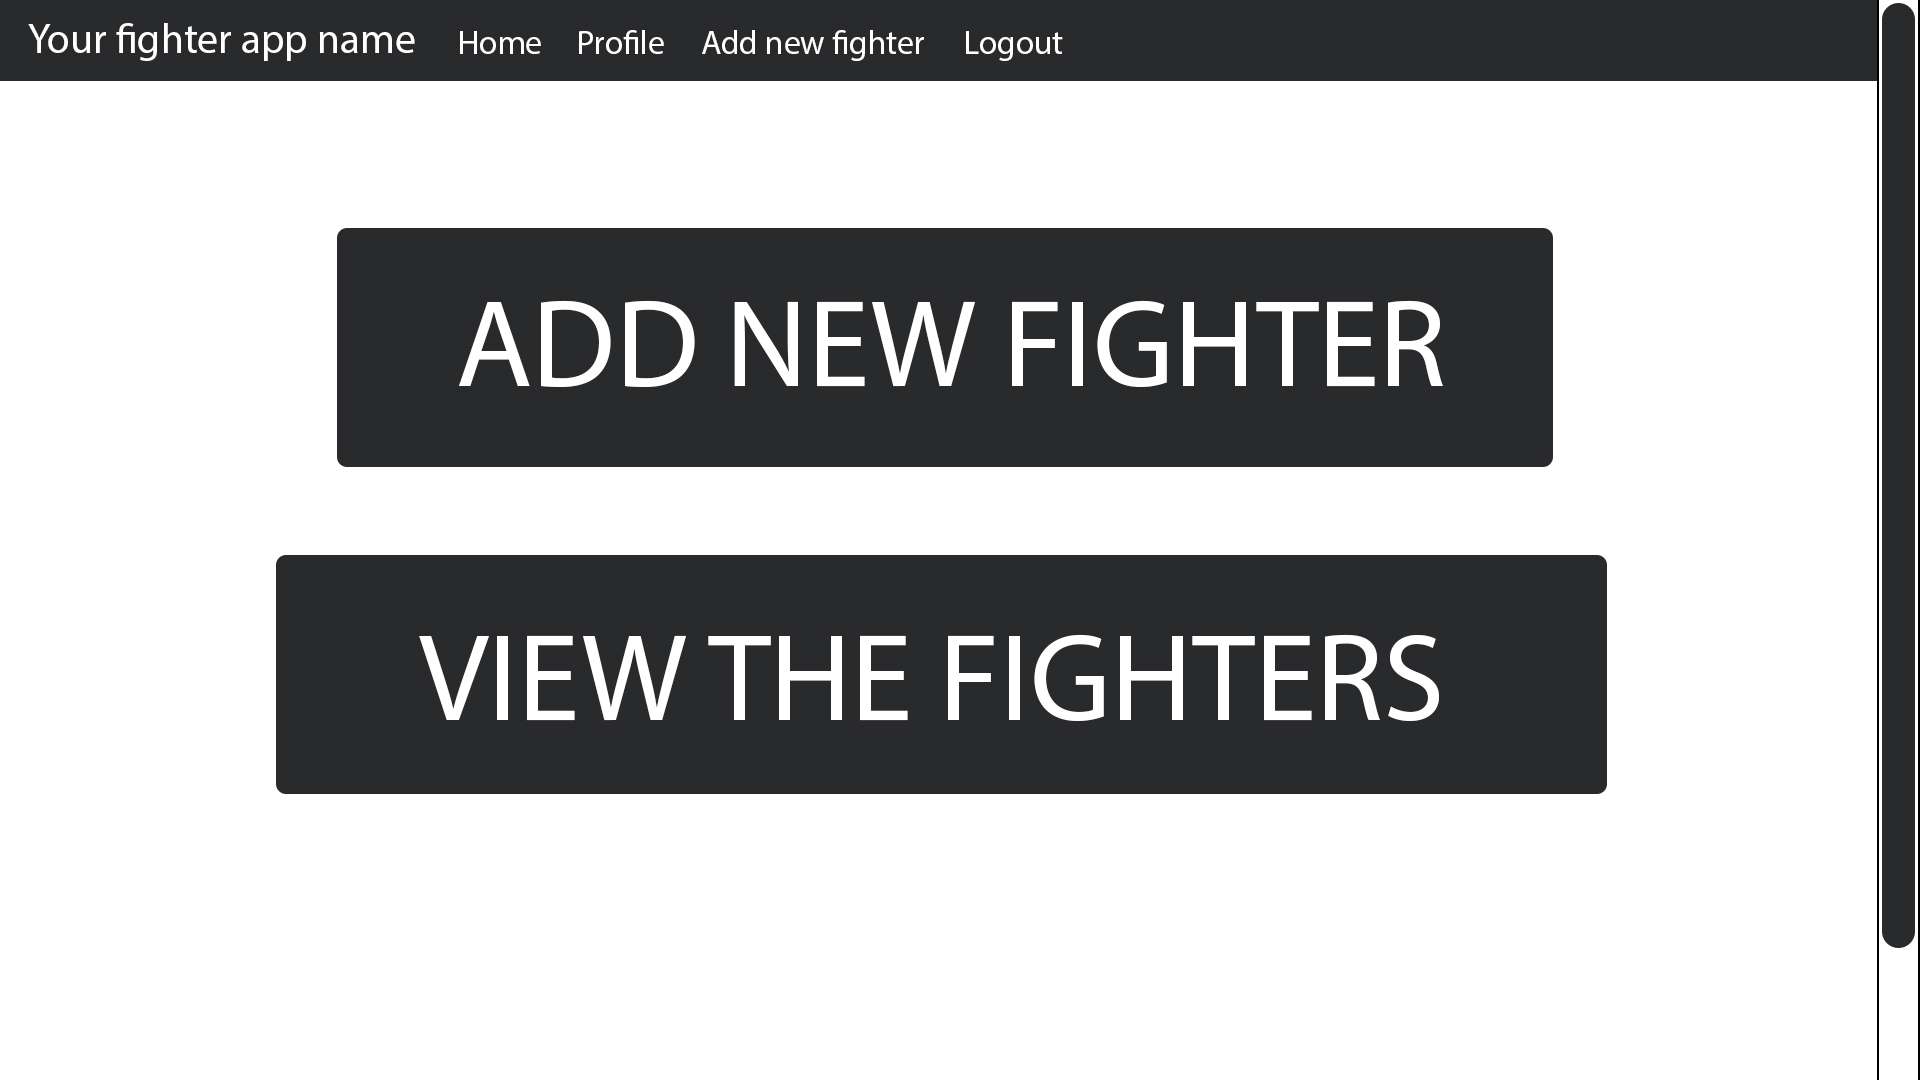
\includegraphics[scale=0.2]{kepek/new_fighter.jpeg}
\caption{Főoldal (Home)}
\label{fig:new_fighter}
\end{figure}

A VIEW THE FIGHTERS nevezetű linkre kattintva a /fighters oldal jelenítődik meg a harcosok listájával (\ref{fig:search_bar}. ábra).

\begin{figure}[htb]
\centering
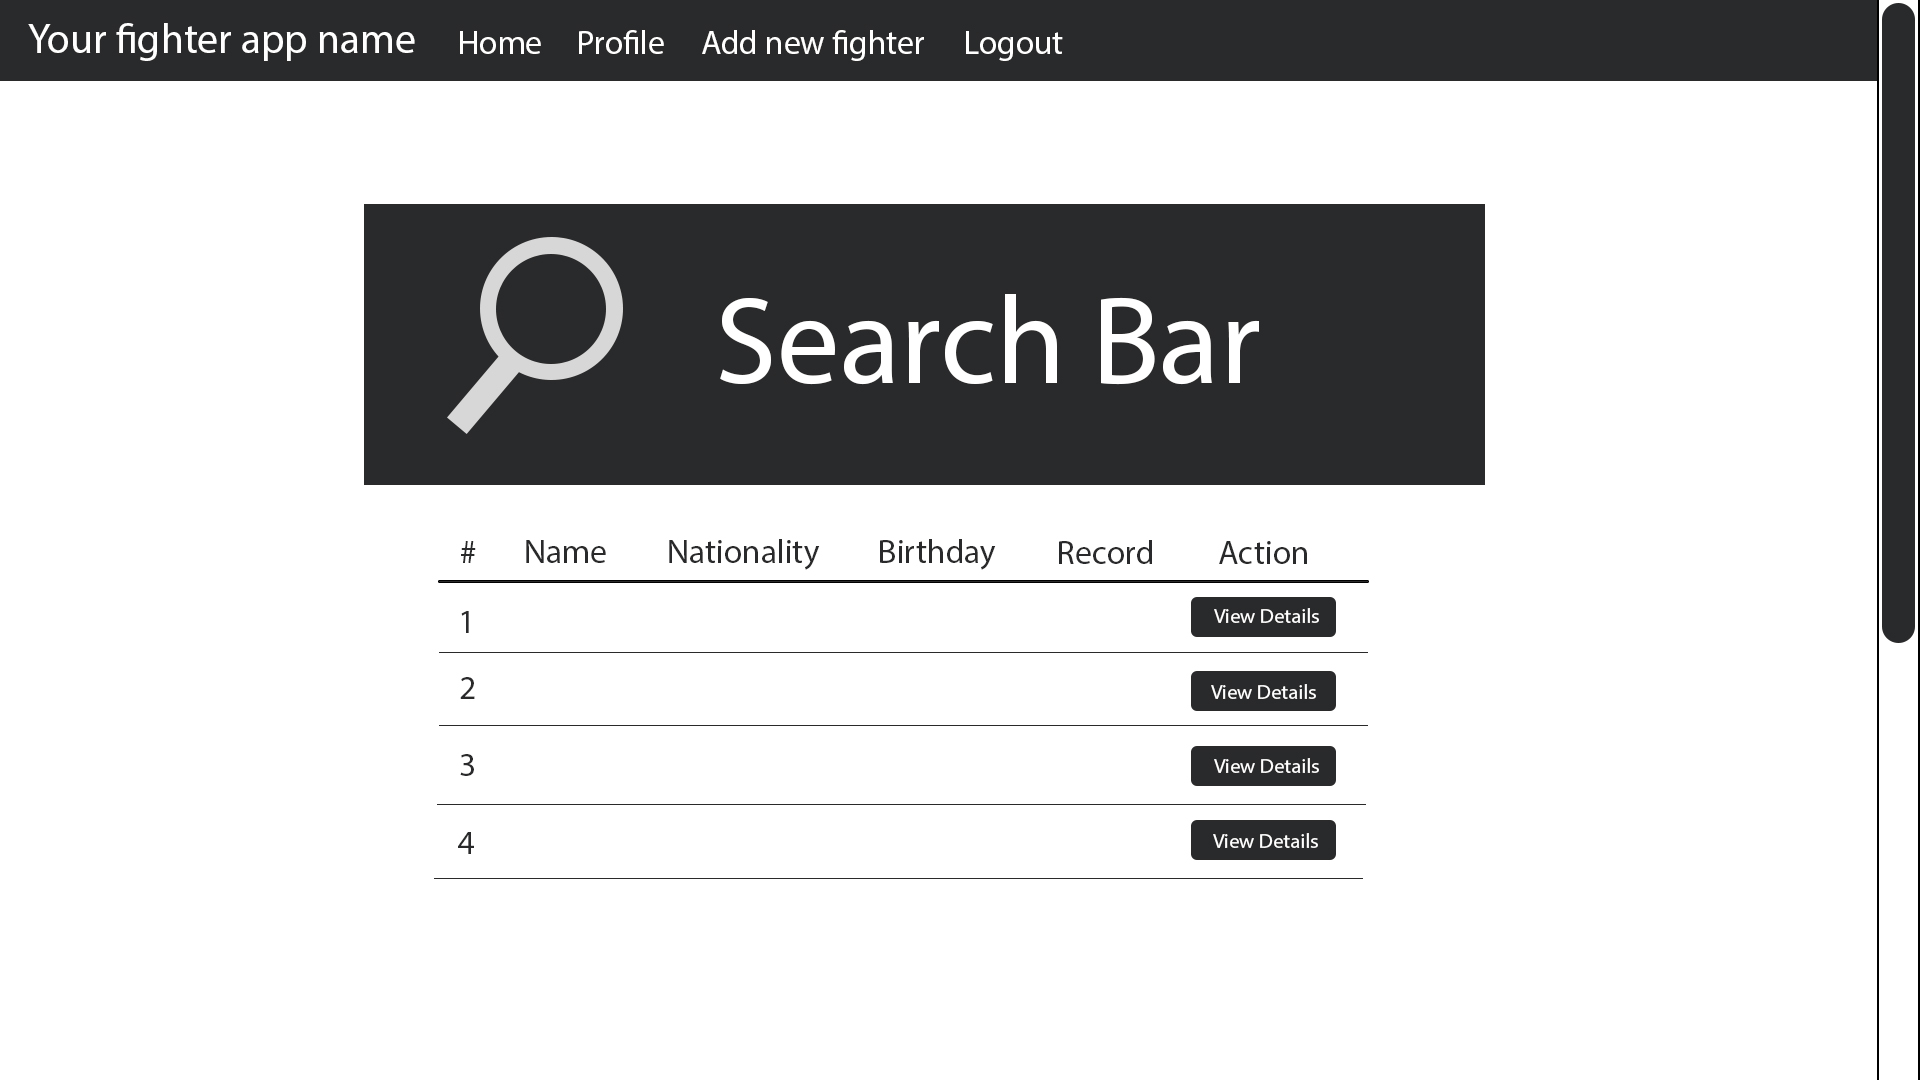
\includegraphics[scale=0.2]{kepek/search_bar.jpeg}
\caption{Harcos lista oldal (Fighters)}
\label{fig:search_bar}
\end{figure}

A harcos sorában lévő View Details feliratú linkre kattintva az adott harcos adatait tartalmazó oldal jön be /fighters/details/id formában (\ref{fig:details}.

\begin{figure}[htb]
\centering
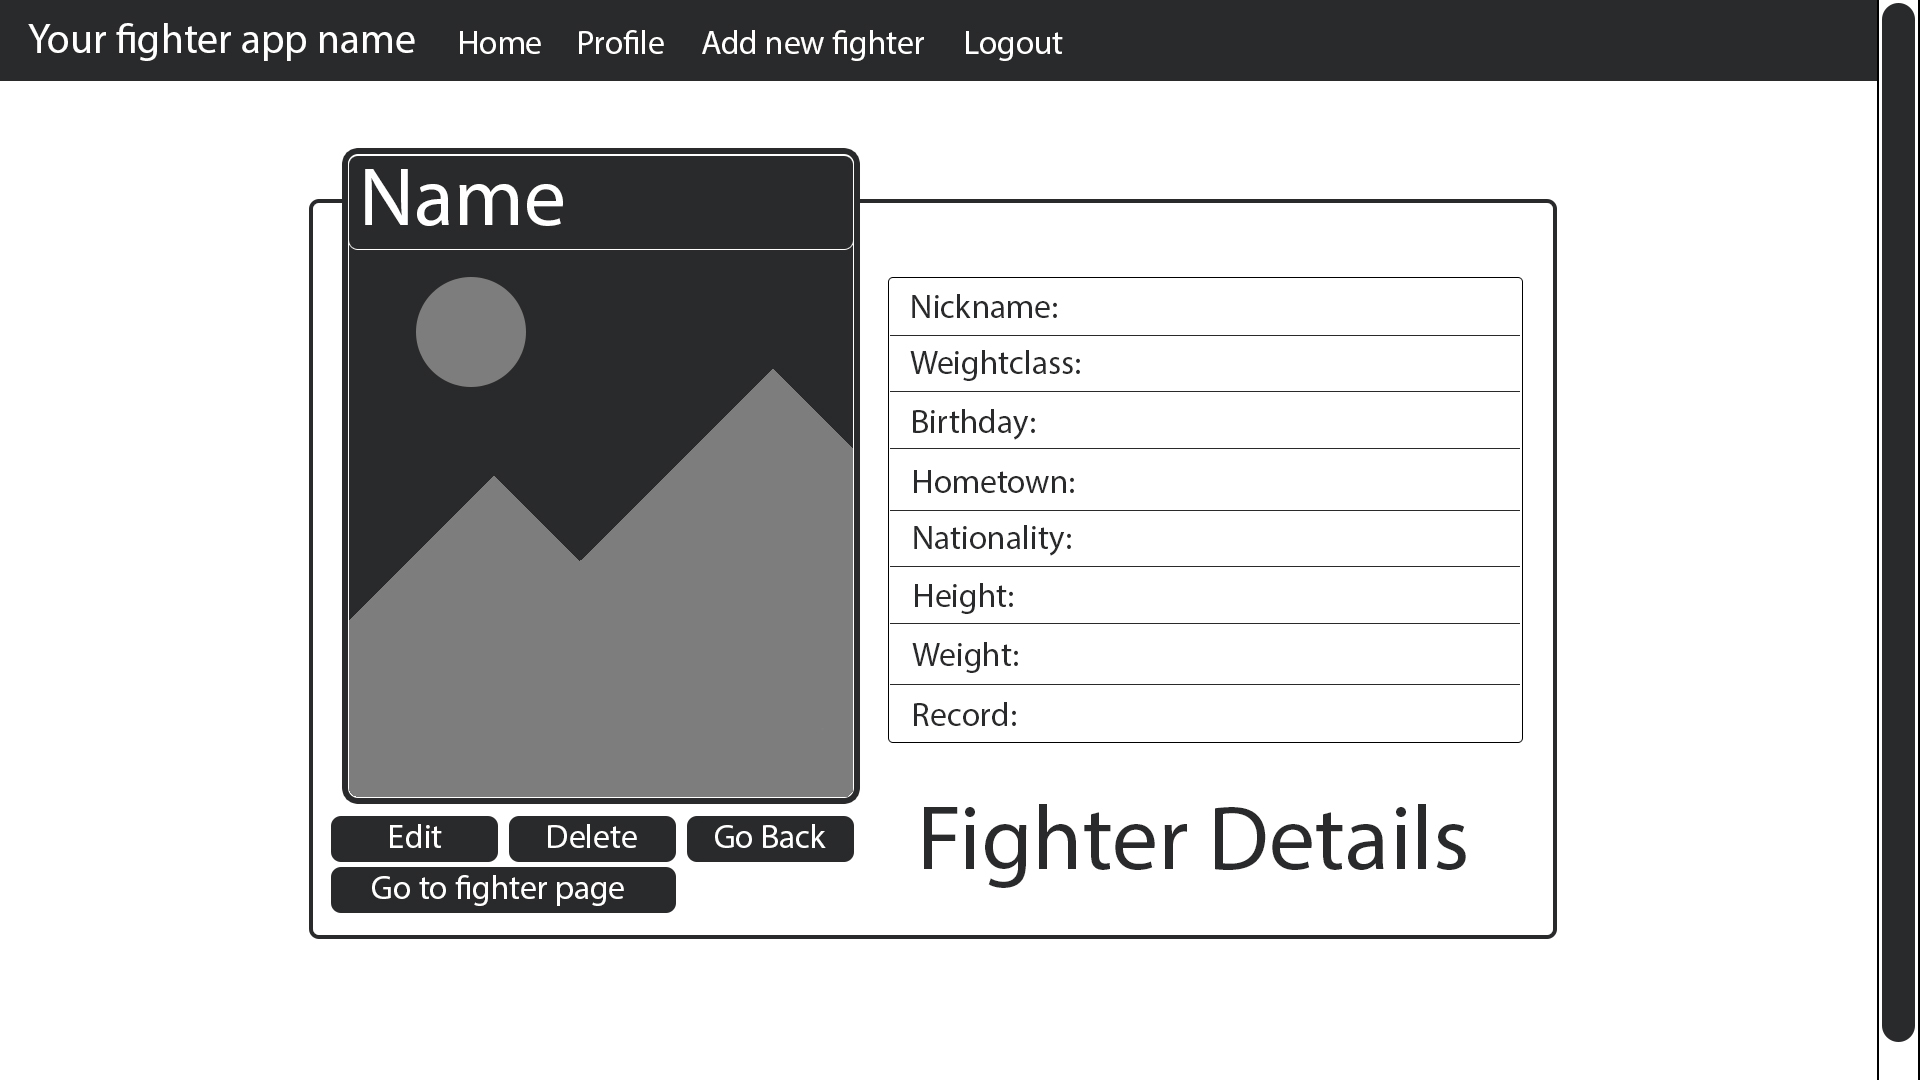
\includegraphics[scale=0.2]{kepek/details.jpeg}
\caption{Harcos adatait megjelenítő oldal (Fighter Details)}
\label{fig:details}
\end{figure}
